\documentclass[%
 reprint,
%superscriptaddress,
%groupedaddress,
%unsortedaddress,
%runinaddress,
%frontmatterverbose,
%preprint,
%showpacs,preprintnumbers,
%nofootinbib,
%nobibnotes,significance, quality, and general
%bibnotes,
 amsmath,amssymb,
 longbibliography,
 aps,
%pra,
%prb,
%rmp,
%prstab,
%prstper,
%floatfix,
]{revtex4-1}

\usepackage[normalem]{ulem}
\usepackage{graphicx}% Include figure files
\usepackage{bm}% bold math
\usepackage{xcolor}
\usepackage{hyperref}
\usepackage{amsmath}
\usepackage[utf8]{inputenc}
\newcommand{\ec}[1]
{\textcolor{red}{[#1]}}
\graphicspath{{Figures/}}

\begin{document}

\title{Anomalous Fluctuations of Extremes in Many-Particle Diffusion}
\author{Jacob B Hass}
\affiliation{Department of Physics and Materials Science Institute, University of Oregon, Eugene, Oregon 97403, USA.}
\author{Aileen Carroll-Godfrey}
\affiliation{Department of Physics and Materials Science Institute, University of Oregon, Eugene, Oregon 97403, USA.}
\author{Ivan Z Corwin}
\affiliation{Department of Mathematics, Columbia University, New York, New York 10027, USA.}
\author{Eric I Corwin}
\affiliation{Department of Physics and Materials Science Institute, University of Oregon, Eugene, Oregon 97403, USA.}
\date{September 2021}

\begin{abstract}
Over one hundred years ago Einstein created a remarkably simple and powerful theory describing the behavior of a single diffusing particle. That theory has since been applied countless times to successfully model widely disparate systems. However, this theory neglects the effects a shared environment has on the particles. As a consequence, the Einstein theory dramatically fails to predict the behavior of extreme diffusion, i.e. outlier particles which have moved the farthest from their starting points. We study particles undergoing a random walk in a beta distributed environment and provide theoretical predictions, which we confirm numerically, of the behavior of the maximally displaced particle. By introducing a shared environment, we find three scaling regimes relating to the KPZ equation for the variance of the maximally displaced particle, contrary to the Einstein diffusion model which predicts a single scaling regime. Understanding the behavior of outliers will have wide ranging applicability to physical, biological, epidemiological, economic, and social systems where outliers often determine behavior.
\end{abstract}

\maketitle

\section{Outline}

\begin{enumerate}
    \item Introduction
    \item Background (Einstein, which in our language is a deterministic CDF calculation plus a Gumbel-ish process)
    \item Discrete model for diffusion, how to compute the CDF from it, how to compute the maximum value from it
    \item Computational methods to implement this model
    \item What is already known about this particular discrete model (asymptotics in large and moderate deviations)
    \item Convert known results in large and moderate deviations into $log(N)$, $log(N)^2$ language)
    \item Matching the two regions together
    \item Sample the CDF: computing the actual max by including the Gumbel (already described in Background).  Explicitly compute it.
    \item Results, comparisons of numerics to theory and to pure Einstein, across broad range of N
\end{enumerate}

\section{Introduction}
Understanding outliers is the key to describing many important phenomena, including biological processes dependent on the interactions between strands of DNA, patient zero spreading a virus to a new area in a pandemic, many chemical processes, and how microscopic price fluctuations relate to long-term macroscopic trends in the stock market \cite{label1, label2, label3, label4}. How do we predict the behavior of these outliers? In diffusive environments, where many particles spread outward from their originating source, we can use Einstein’s theory of diffusion to describe the bulk behavior of the particles \cite{label5, label6}. Einstein described diffusion as particles undergoing independent random walks. The random-walk description ignores the effect the shared environment has on the particles, resulting in its potential failure to correctly describe the diffusion of the outliers. Particles near each other should be influenced by the medium in the same way, but in Einstein’s theory of diffusion, their behavior is totally independent from one another. As a result, when analyzing the system as a whole, the distributions of outlier particle locations and first passage times will differ from that predicted by Einstein’s theory. The objective of this work is to show this discrepancy and demonstrate the need for a new theory of extreme diffusion. \par
We study the behavior of the maximally displaced particle undergoing a 1D random walk in a beta distributed environment. Einstein's model of diffusion predicts the variance of the maximally displaced particle to grow proportionally to time. Additional theories of diffusion have been introduced with variances that scale with $t^{\alpha}$ for $\alpha>1$, super-diffusive, or $\alpha<1$, sub-diffusive. By studying particles moving in beta distributed environments, we found three scaling regimes which depend on the underlying beta distribution.

\section{Background}

\section{Discrete Systems}

\begin{figure}[h]
  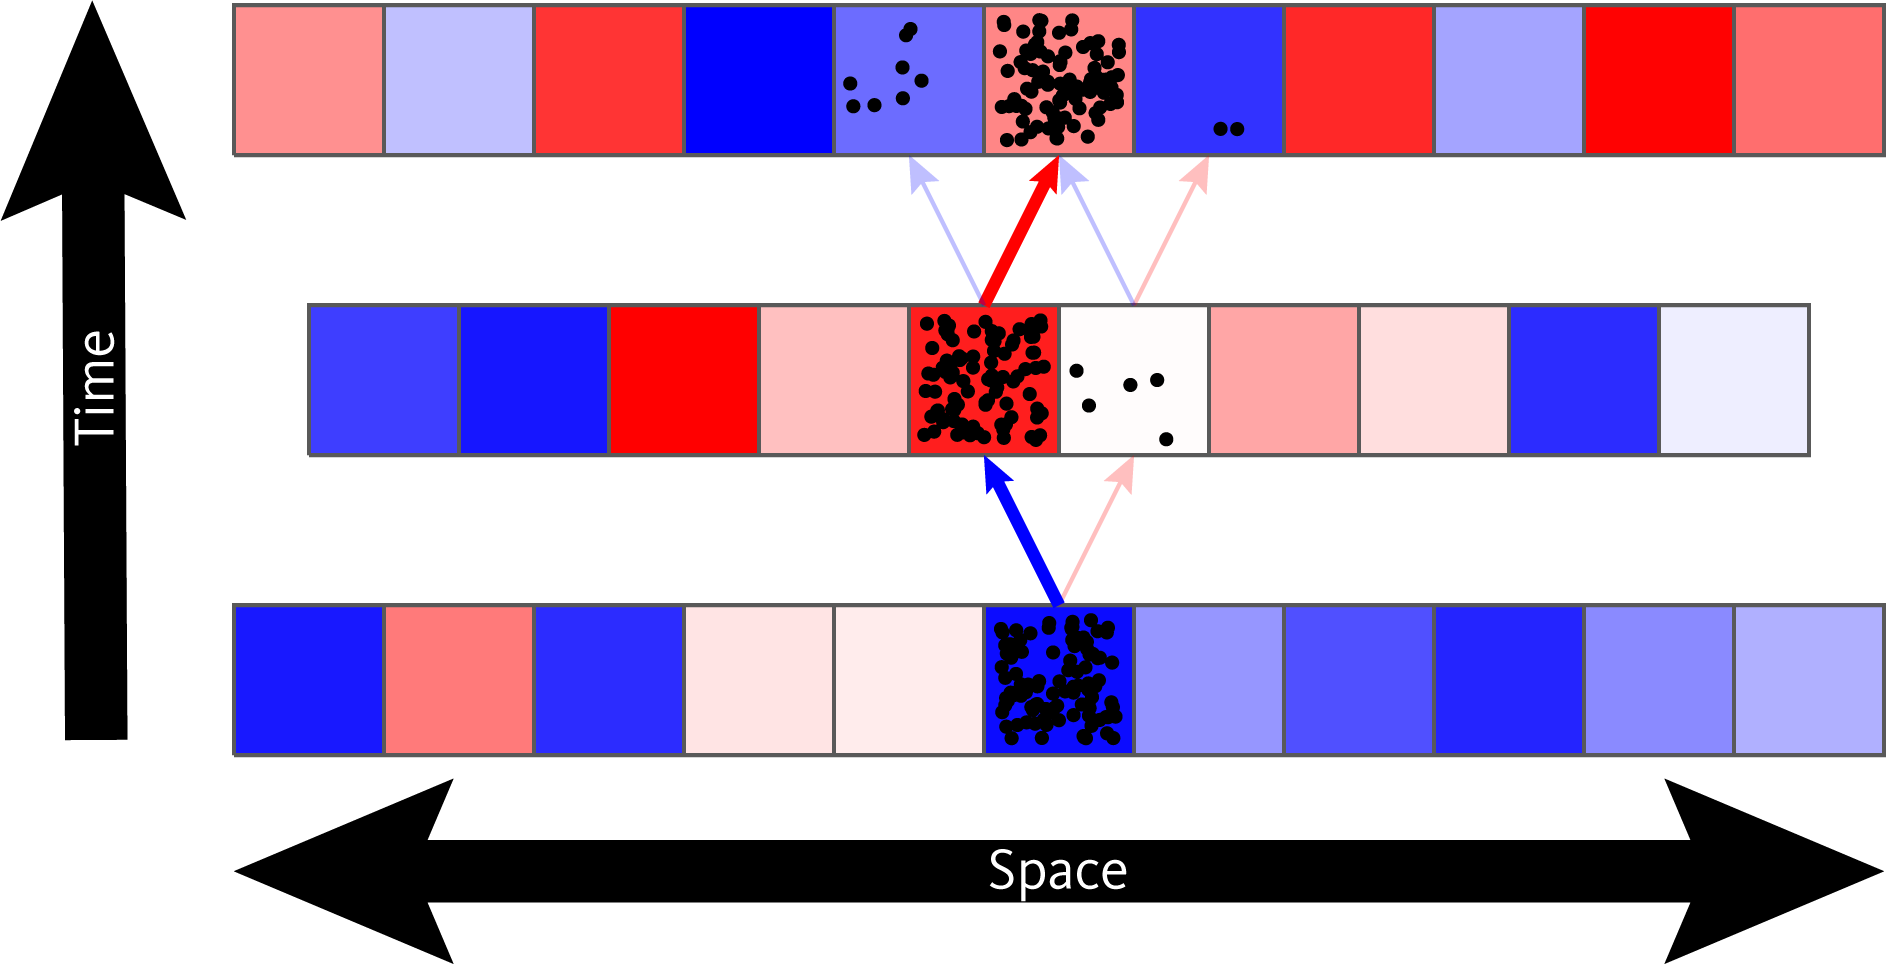
\includegraphics[width=\columnwidth]{BCModel1d.png}
\end{figure}

\begin{figure}[h]
  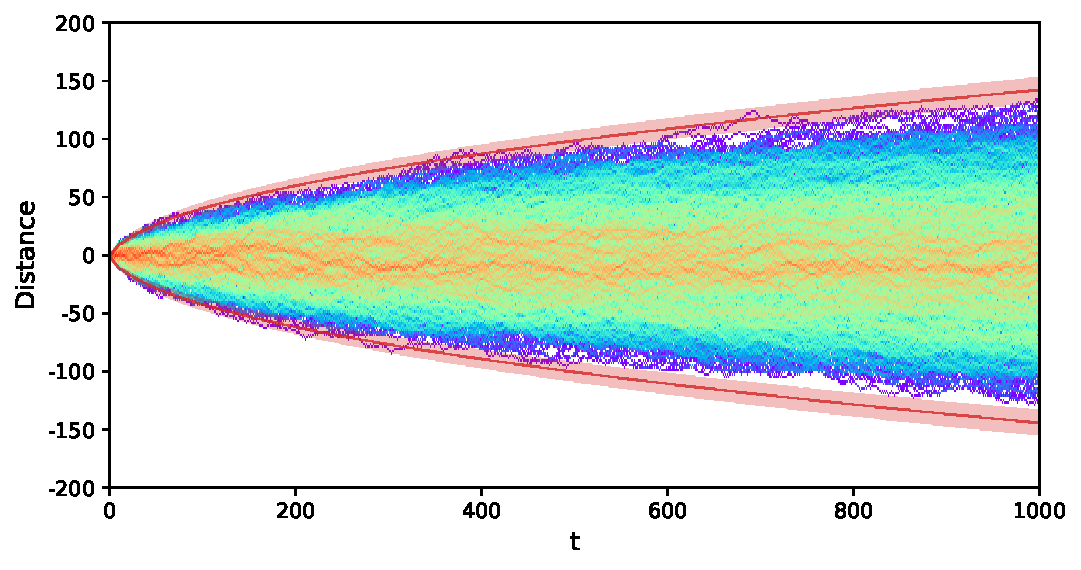
\includegraphics[width=\columnwidth]{Occupation.png}
  \caption{System over time}
\end{figure}

\section{Computational Methods}
We compute the PDF using quad precision numbers.

Different binomial distribution approximations.

\section{Asymptotics in large and moderate deviations}
\section{The $log(N)$ and $log(N)^2$ regimes}
\section{Matching two regions}
\section{Sampling the CDF}
\section{Results}

\begin{figure}[h]
  \includegraphics[width=\columnwidth]{DiscreteMean.png}
  \caption{Mean max particle over time}
\end{figure}

\begin{figure}[h]
  \includegraphics[width=\columnwidth]{DiscreteVariance.png}
  \caption{Max particle variance over time}
\end{figure}

\begin{figure}[h]
  \includegraphics[width=\columnwidth]{PDFVariance.png}
  \caption{Quantile variance over time}
\end{figure}

\begin{thebibliography}{30}

\bibitem{label1} Yaojun Zhang and Olga K. Dudko. First-Passage Processes in the Genome. Annual Review of Biophysics,

\bibitem{label2}  L. Hufnagel, D. Brockmann, and T. Geisel. Forecast and control of epidemics in a globalized world. Proceedings of the National Academy of Sciences, 101(42):15124–15129, October 2004. Publisher: National Academy of Sciences Section: Biological Sciences.

\bibitem{label3}  Sidney Redner. 8. Applications to Simple Reactions. In A Guide to First-Passage Processes, pages 252–294. Cambridge University Press, Cambridge, 2001.

\bibitem{label4}  Hsing Liu, Chi-Yo Liao, Jing-Yuan Ko, and Jiann-Shing Lih. Anchoring effect on first passage process in Taiwan financial market. Physica A: Statistical Mechanics and its Applications, 477:114–127, July 2017.

\bibitem{label5}  A. Einstein. Über die von der molekularkinetischen Theorie der Wärme geforderte Bewegung von in ruhenden Flüssigkeiten suspendierten Teilchen. Annalen der Physik, 322(8):549–560, January 1905.

\bibitem{label6}  M. von Smoluchowski. Zur kinetischen Theorie der Brownschen Molekularbewegung und der Suspensionen. Annalen der Physik, 326(14):756–780, 1906.

\bibitem{label7}  Guillaume Barraquand and Ivan Corwin. Random-walk in Beta-distributed random environment. Probability Theory and Related Fields, 167(3-4):1057–1116, April 2017.

\end{thebibliography}

\end{document}
